\chapter[Xenon Mobility in \protect\NoCaseChange{U--Mo} fuel]{Xenon Mobility in BCC-Uranium and Uranium--Molybdneum Alloys}
\textit{This chapter is based on work that will be submitted for publication to the Journal of Physics: Condensed Matter. The authors are A. Rafi M. Iasir and Karl D. Hammond of the University of Missouri.}



\section{Introduction}\label{sec_intro}
High performance research reactors require high-enrichment uranium (HEU) fuels
to attain the desired neutron flux. The replacement of HEU fuels with
low-enrichment uranium (LEU) is an important antiproliferation initiative. The
United States High-Performance Research Reactor (USHPRR) program is currently
aiming to replace the HEU fuels currently used in high performance reactors
with LEU fuels~\cite{snelgrove1997development}.
LEU fuels require a higher uranium density than that of uranium oxides
to compensate the decrease in \ce{^{235}U} enrichment.
Metallic uranium shows a great promise in this regard.

Metallic fuels are usually chosen because of their high thermal conductivity
and high density. Isotropic swelling behaviour is desirable, but uranium,
like other light actinides (Pa--Pu), has a low-symmetry crystal structure
(the orthorhombic \textalpha\ phase) at ambient temperature and pressure,
which results in anisotropic thermal and radiation-induced expansion.
%The influence of $5f$ electron--electron correlation plays an
%important role in the crystal structure of uranium and other light
%actinides~\cite{Soderlind1995,lander2003gh, freemanHandbook1984}.
%A narrow band of $5f$ states ($\approx$\,1--3~eV) goes through Peierls
%distortions~\cite{peierls1955} and favours an open, low-symmetry structure.
Pure uranium has three allotropes at atmospheric pressure:
\textalpha\ (base-centred orthorhombic), \textbeta\ (tetragonal), and
\textgamma\ (body-centred cubic). At atmospheric pressure, \mbox{\textalpha-U}
transforms to \mbox{\textbeta-U} at approximately 935~K, and \mbox{\textbeta-U}
transforms to \mbox{\textgamma-U} at approximately
1045~K~\cite{lawson1988structure,akella1997structural}. 

The \mbox{\textgamma-uranium} allotrope (which is body-centred cubic) is
preferred to \mbox{\textalpha-uranium} by nuclear engineers because it
undergoes both isotropic thermal expansion and isotropic radiation-induced
swelling~\cite{kittel1993history}.
It is not possible to quench pure \mbox{\textgamma-uranium} to room
temperature; however, a metastable bcc phase can be obtained at room
temperature by alloying with
molybdenum~\cite{wilson1949structures, sinha2010phase,
    yakel1969crystal,sinha2010effect}.
A study by Kim-Ngan and Havela~\cite{kim2016superconductivity} showed that the
bcc structure can also be retained at temperatures below the ordinary phase
transition temperature by alloying uranium with metals such as platinum,
palladium, niobium, and zirconium.
Molybdenum stabilises uranium's \textgamma\ phase at concentrations near the
eutectoid point (11.1 wt\% Mo) and lowers the phase transition temperature from
1045~K for pure \textgamma-uranium to 828~K for a U--Mo alloy at the eutectoid
point~\cite{ASM-Alloy-Mo,Berche2011}.
Uranium alloyed with 10~wt\% molybdenum (U-10Mo, which is approximately
21.6~at.\% molybdenum) is currently being developed as a potential
high-density, low-enrichment uranium fuel for high-performance research
reactors~\cite{prabhakaran2017u, meyer2014irradiation, williams2017post}.

Uranium--molybdenum alloys have been studied extensively both
experimentally~\cite{dwight1960uranium,tangri1961metastable, sinha2010phase}
and theoretically~\cite{berche2011calphad,zhang2010thermodynamic,
    losada2019ground, landa2011density,alonso2007role}.
Castellano \etal~\cite{castellano2020thermodynamic} showed that the
addition of molybdenum to uranium leads to the stabilisation of the
\textgamma\ phase using \textit{ab initio} molecular dynamics.
This thermodynamic stabilisation is important because un-alloyed
\textgamma-uranium would quickly revert back to \textalpha-uranium, causing high stresses and
cracking of the fuel and cladding. %The transition to $\alpha + \text{U}_2\text{Mo}$ happens more quickly in the irradiation environment.

Fission creates a variety of products, resulting in gas bubbles,
metallic precipitates, and solutes in the fuel matrix.
Among the many fission products, fission gas (\ie, xenon and krypton) produces
some of the most significant challenges associated with nuclear fuel
development. Fission gas influences the thermal conductivity,
causes swelling, and impacts the neutron economy of the
reactor~\cite{rondinella2010high,iasir2018estimation}. 

The atomic-scale transport processes in U--Mo alloys are of great interest to
understand fuel performance during irradiation.
%Interestingly, molybdenum is itself a fission product.
Specifically, the characteristics of fission gas are an important
performance-limiting factor. For these reasons, the behaviour of fission gas
has been extensively researched for common fuels such as
\ce{UO2}~\cite{yun2008atomic,carter1972xenon,matzke1966diffusion,
    macewan1964xenon, une1987effects}.
A number of theoretical approaches have also been used to understand the
behaviour of fission products in \ce{UO2}, including electronic structure
theory~\cite{catlow1978fission,jackson1986calculation,grimes1989calculations,
    ball1990diffusion,grimes1991stability, petit1999location,
    crocombette2002ab, freyss2006ab, andersson2011u}.
In particular, vacancies play an important role in the diffusion of xenon
because of its size relative to the metal atoms.

Solute diffusion in light actinides is a very interesting phenomenon because
such solutes typically have very high diffusivities.
% FIXME Relative to...? Uranium self-diffusion?
Diffusion of solutes in metallic uranium has not been studied extensively.
However, there are some early works that provide some information about defect
and impurity diffusion in uranium~\cite{adda1959etude,peterson1964diffusion,
    rothman1959self, rothman1961diffusion, adda1962etude, resnick1962self,
    rothman1961self, liu2012atomic}.
Recently, Smirnova \etal~\cite{smirnova2015atomistic} studied self-diffusion in
\textgamma-uranium and U--Mo alloys using molecular dynamics.
They showed that diffusion in \textgamma-uranium is anomalously fast compared
to other bcc metals.

In recent years, there have been many attempts to calculate diffusion
coefficients using electronic structure and atomistic
methods~\cite{adams1989self, blochl1993first, blochl1990first, frank1996first,
    janotti2004solute, krvcmar2005diffusion, milman1993free, sandberg2002self}.
Electronic structure calculations based on DFT and multi-frequency models have
shown their usefulness in various works.
Five-frequency models of face-centred cubic
    crystals~\cite{lidiard1955,lidiard1960, leclaire1956} and
nine-frequency (or sometimes four-frequency) models of bcc
crystals~\cite{leclaire1970, mehrer2007diffusion} have been widely used.
Methods based on electronic structure theory involve calculating the activation
energies of an atom jumping to a vacancy in one of the atom's nearest-neighbour
positions. This is often referred to as vacancy-mediated diffusion.
The calculations employed here are based on DFT coupled with classical
transition state theory (TST), which treats vibration using the
harmonic oscillator
approximation~\cite{vineyard1954theory, vineyard1957frequency}.

In this study, we use DFT and TST to study the diffusion of xenon and
molybdenum in \textgamma-uranium alloys such as U--7Mo and U--10Mo by varying the local molybdenum concentration around the diffusing solute atom.
We find that molybdenum's migration energy is much higher than xenon's in
\textgamma--U alloys and that the presence of molybdenum in the local
environment of a xenon atom tends to
decrease the mobility of xenon in \textgamma-uranium alloys.
We also calculate the vacancy--solute binding energies of several solutes
in \textgamma-uranium and find that such binding energies are generally
higher in \textgamma-uranium than in iron or aluminium.

\section{Thermodynamics of Vacancies in Solid}

\section{Theory}\label{sec_theory}
Diffusion coefficients in crystalline solids are often described by an
Arrhenius equation over a wide range of temperatures. This model consists of
two parameters, the migration energy, $E_m$, and the pre-exponential factor,
$D_0$, with the diffusion coefficient given by
\begin{equation}
    D = D_0 e^{-E_m/k_B T},
\end{equation}
where $k_B$ is the Boltzmann constant and $T$ is the absolute temperature.
If $D_0$ is independent of temperature, an Arrhenius plot ($D$ against $1/T$)
gives a straight line; if $D_0$ changes with $T$, it yields a curve that falls
away from the constant-$D_0$ line at high temperature (the left of the plot).

The migration energy is the activation energy for an atom to jump onto a
nearby vacancy. According to classical transition state theory (TST), the rate
at which a vacancy exchanges its place with neighbouring atom can be expressed
by the Eyring--Polanyi
equation~\cite{Eyring1935,Evans1935,vineyard1957frequency},
\begin{equation}
    v = \nu^\ddagger \exp\left(\frac{-\Delta G_m}{k_B T}\right)
      \approx \frac{k_B T}{h} \frac{Q_\text{TS}}{Q_\text{IS}}
              \exp\left(\frac{-E_m}{k_B T}\right)
      \approx \frac{k_B T}{h}
              %\left[
              %\frac{\displaystyle\prod_{i=1}^{3N-3} \nu_i}
              %     {\displaystyle\prod_{j=1}^{3N-4} \nu_j^\ddagger}
              %\right]
              \exp\left(\frac{-E_m}{k_B T}\right),
\end{equation}
where $Q_\text{IS}$ is the vibrational partition function of the initial
state and $Q_\text{TS}$ is the vibrational partition function of the transition
state with the vibrational mode along the minimum-energy pathway removed.
In the current work, we did not calculate the jump frequencies, which are
part of the $Q_i$ terms; we instead make the approximation that the vibrational
partition functions not associated with the minimum energy pathway are unity
(\ie, $Q_\text{TS}/Q_\text{IS} \approx 1$).
The diffusion coefficient is proportional to the rate of a jump:
$D = v\lambda^2/6,$ where $\lambda = a/\sqrt{8}$ for bcc
lattices~\cite{Heinola2010a} and $a$ is the lattice parameter.


Metals that undergo irradiation produce point defects such as self-vacancies and self-interstitials in the lattice. The diffusion of these defects results in microstructural changes that impact the mechanical properties. The diffusion of vacancies is of significant interest because they form voids, dislocation loops, and clusters, and they facilitate the diffusion of substitutional solute atoms. This method of solute diffusion is controlled by the interaction between a vacancy and a solute atom. The diffusion of vacancies is particularly influenced by the presence of nearby substitutional solute atoms. Sometimes the vacancy and the solute can coexist as an atom--vacancy complex. Hence, understanding solute--vacancy interactions is an important step in developing models of diffusion in irradiated materials.
%Several factors influence impurity diffusion dueto the interaction between the impurity atom and the vacancy. 
The binding energy between vacancies and solute atoms is a key factor in understanding solute 
diffusion~\cite{balluffi1973diffusion, wolverton2007solute}. Nearby solute atoms
can influence the energy of solute binding with vacancies. The authors are not aware of any previous results regarding solute--vacancy
binding in \textgamma-uranium for any solutes, so we calculated them as part of
this work.

We used defects in supercells to calculate the binding energies
of solute--vacancy (\ce{$X$-$\Box$}) pairs. The binding energy is the
difference between the energy at infinite separation and the energy at
nearest-neighbour separation. We used the following expression to calculate the
binding energy of a solute to a vacancy:

\begin{equation}
  E_\text{bind}^{\ce{$X$-\Box}}
    = E^{X_1}_{\mathrm{U}_{N-1}} + E^{\Box_1}_{\mathrm{U}_{N-1}}
    - E^{X_1\Box_1}_{\mathrm{U}_{N-2}} - E_{\mathrm{U}_N}
  \label{eq_solvacen}
\end{equation}

For a bcc supercell with $N$ sites, the cell may contain no defects (energy
$E_{\mathrm{U}_N}$), may contain a vacancy (energy $E^{\Box_1}_{\mathrm{U}_{N-1}}$), a solute
impurity ($E^{X_1}_{\mathrm{U}_{N-1}}$ or a solute--vacancy pair
($E^{X_1\Box_1}_{\mathrm{U}_{N-2}}$).
%The negative sign in Eq.~\eqref{eq_solvacen} is
%to keep the binding energy consistent with the literature, where 
A positive binding energy means the complex is bound.
Equation~\eqref{eq_solvacen} can
also be conveniently written as the energy required to form a vacancy next to
a solute ($X$) atom. The vacancy formation energy is 
\begin{equation}
    E^{\Box}_f = E^{\Box_1}_{\mathrm{U}_{N-1}}
        - \frac{N-1}{N} E_{\mathrm{U}_N},
  \label{eq_vacen}
\end{equation}
where $E_{\mathrm{U}_N}$ is the energy of a supercell with $N$ uranium atoms.

The disordered nature of U--Mo alloys creates some challenges for electronic
structure studies. The manner in which molybdenum is distributed among the
uranium atoms produces different diffusion pathways
for xenon, and there are several ways to arrange molybdenum atoms on the
lattice sites around a xenon atom. We use a combinatorial approach to assess
the probabilities (Table~\ref{tab_combination}) of having various numbers of
molybdenum atoms in the first-nearest-neighbour shell of the bcc structure
around a xenon atom. Assuming the molybdenum atoms are arranged randomly, the
probability of a particular U/Mo combination on the sites near a xenon
atom can be calculated using the following equation:
\begin{equation}\label{eq_combination}
  \mathcal{P} = \binom{n}{k} x^k_\text{Mo} ( 1 - x_\text{Mo})^{n-k},
\end{equation}
where $n$ is the number of available nearest-neighbour positions not occupied
by the vacancy (for bcc, $n=7$), $k$ is the number of molybdenum atoms in
the nearest-neighbour shell, and $x_{\ce{Mo}}$ is the (overall) mole fraction
of molybdenum. According to Table~\ref{tab_combination},
the probability ($\mathcal{P}$) of having more than three molybdenum atoms in
the first nearest-neighbour shell is low ($< 5\%$).
We assume, for simplicity, that $x_{\ce{Xe}} \approx 0$.

\begin{table}
	\centering
    \caption{Probability of having different numbers of molybdenum atoms in the
        nearest-neighbour (NN) location for a bcc uranium--molybdenum alloy.
        We have used Eq.~\eqref{eq_combination} to calculate the probabilities.}
	\label{tab_combination}
	\begin{tabular}{ccc} \toprule
        & U--10Mo & U--7Mo \\
      \# of Mo & ($x_\text{Mo}$ = 0.216) & ($x_\text{Mo}$ = 0.157) \\ \midrule
		0 & 0.182 & 0.302 \\ 
		1 & 0.351 & 0.394 \\
		2 & 0.290 & 0.221 \\
		3 & 0.133 & 0.069 \\
		4 & 0.037 & 0.013 \\
		5 & 0.006 & 0.001 \\
		6 & 0.0006 & \num{8.95e-05} \\
		7 & \num{2.19e-05} & \num{2.39e-06} \\ \bottomrule
	\end{tabular}
\end{table}

\section{Methodology}\label{sec_method}


All calculations used the \textsc{Quantum ESPRESSO}~\cite{giannozzi2009quantum}
simulation package with the projector-augmented wave (PAW)
method~\cite{Bloechl1994}. A full description of the uranium pseudopotential
can be found in our earlier work~\cite{iasir2020pseudopotential}.
For the elements Mo, Xe, Fe, Co, Au, Nb, and Zr, we used PAW-based
pseudopotentials from the \textsc{Quantum ESPRESSO}
PS Library~\cite{pp1,dal2014pseudopotentials}. We used the
exchange--correlation functional of Perdew, Burke, and Ernzerhof
(PBE)~\cite{Perdew1996b,Perdew1997} for all calculations.

DFT calculates the ground state properties of a system;
however, \textgamma-uranium is mechanically unstable at 0~K, which results in
negative shear moduli~\cite{soderlind1998theory}.
Other elements (\eg, Ti, Zr, Pr, and Hf)
also have high-temperature bcc structures that are unstable at low
temperature~\cite{ye1987phonon,sanchez1975model}. 
It is consequently challenging to study \textgamma-uranium with DFT,
particularly using a supercell that includes vacancies or defects.
To perform our calculations, we used the so-called shell
method~\cite{beeler2010first}, in which the outer layer of atoms is fixed at
crystallographic coordinates and the rest of the atoms are allowed to move
freely.
We used a $3\times3\times3$ supercell of bcc uranium, which consists of 54
atoms in the absence of heteroatoms or vacancies.
A convergence test showed that a Monkhorst--Pack $k$-point mesh of
$5\times5\times5$ is suitable to yield formation and migration energies
that are converged to within 0.01~eV\AA$^{-1}$.

To calculate the migration energy, each initial state was relaxed with respect
to internal coordinates and volume. We determined the transition state by way
of a nudged elastic band (NEB)~\cite{henkelman2000climbing,
    henkelman2000improved}
calculation with a climbing image as implemented in \textsc{Quantum ESPRESSO}. We used five images in the NEB calculations.

\section{Results and Discussion}\label{sec_result}
\subsection{Vacancy Formation and Impurity--Vacancy Binding Energies}

The formation energy of a single vacancy is calculated using
Eq.~\eqref{eq_vacen}. Our results are compared with previously-published DFT
calculations and experimental results in Table~\ref{tab_vacen}.
Our results are in good agreement with both previous DFT studies.
Xian \etal~\cite{xiang2008quantum} also used 54 atoms in their supercell, but
our vacancy formation energy is higher by 0.2~eV\@. Discrepancies could arise from
their use of a $6\times6\times6$ $k$-point mesh, whereas we used
$5\times5\times5$. Beeler \etal~\cite{beeler2010first} used a supercell of 128
atoms to calculate the vacancy formation energy. 
The experimental values bracket our results and those of Beeler
\etal~\cite{beeler2010first}: The earlier work of Matter
\etal~\cite{matter1980investigation} found a formation energy of
$1.2\pm0.3$~eV, whereas Lund \etal~\cite{lund2013vacancy} found
$1.6\pm0.2$~eV\@.

\begin{table}
    \centering
    \caption{Vacancy formation energy (eV) of \textgamma-U compared with
        previously-published results.}
    \label{tab_vacen}
    \begin{tabular}{l l} \\ \toprule
    Source & Energy (eV) \\ \midrule
    Present work & 1.28     \\
    Beeler \etal~\cite{beeler2010first} & 1.384    \\
    Xian \etal~\cite{xiang2008quantum} &    1.08    \\
    Matter \etal\ (expt.)~\cite{matter1980investigation} & $1.2 \pm 0.3$ \\   
    Lund \etal\ (expt.)~\cite{lund2013vacancy} & $1.6 \pm 0.2$  \\ \bottomrule
    \end{tabular}
\end{table}


We are not aware of any previous reports of calculations of solute--vacancy
(\ce{$X$-$\Box$}) binding energies in \mbox{\textgamma-uranium},
so we calculated these ourselves.
We chose solutes so as to compare to diffusion measurements by Rothman and
coworkers~\cite{rothman1961diffusion, rothman1959self, peterson1964diffusion}.
The results are shown in Table~\ref{tab_solvac}.
All of the solute--vacancy binding energies in \mbox{\textgamma-uranium} are
substantially higher than in other bcc metals.
For example, in aluminium and magnesium,
the \ce{$X$-$\Box$} binding energy varies from $-0.4$ to 0.5~eV for a variety
of solutes~\cite{wolverton2007solute, shin2010first,saal2012solute}.
In \mbox{\textgamma-uranium}, however, the binding energy varies from 5.715~eV
(\mbox{\ce{Fe-$\Box$}}) to 6.619~eV (\ce{Cr-$\Box$}),
which indicates that the solute--vacancy binding energy is much higher in bcc
uranium than it is in other bcc metals.

The solute--vacancy binding energy characterizes the interaction between a
solute and a vacancy, which modifies the local concentration of vacancies near
a solute. In the case of \mbox{\textgamma-uranium}, the interaction between
solute and vacancy is strongly attractive.
%Even though the energetic binding between
%solute atoms and vacancies has been studied experimentally and
%theoretically~\cite{raman1971clustering, melikhova2006vacancy,kong2014first,
%wolverton2007solute, simonovic2009impurity, hoshino1996local}, it is still not
%clear how these physical factors influence the solute--vacancy interactions.
The total solute--vacancy binding energy can be decomposed into two factors: 
elastic effects and electrostatic effects~\cite{burke1972measurement}.
The elastic energy (or elastic binding energy) is the energy that is released
if the strain fields of a solute and a vacancy
interact~\cite{kong2014first, ohnuma2009first}.
Due to the unstable nature of \mbox{\textgamma-U} at low temperatures,
the elastic binding energy contributes the most to the total solute--vacancy
binding energy and is the primary reason for the high value of the
solute--vacancy binding energy in bcc uranium. 


\begin{table}
    \centering
    \caption{Solute--vacancy binding energies in \textgamma-uranium for
        various solutes near a vacancy.
        Positive energies indicate energetically-favourable binding.}
    \label{tab_solvac}
    \begin{tabular}{l l}
      \toprule
        Solute & Binding energy (eV) \\
      \midrule
        Xe & 6.034 \\
        Mo & 6.249 \\
        Fe & 5.715 \\
        Co & 5.876 \\
        Au & 6.450 \\
        Cr & 6.619 \\
        Zr & 6.318 \\
        Nb & 6.113 \\
      \bottomrule
    \end{tabular}
\end{table}

\subsection{Xenon and Molybdenum Diffusion}
Migration energies are calculated using the climbing-image nudged elastic band
method. We calculated the migration energies of xenon and molybdenum moving
from the centre of the supercell to one of the nearest-neighbour lattice sites.
Such solute--vacancy exchange is the primary mechanism of diffusion of xenon
and molybdenum because of their size relative to uranium.
Table~\ref{tab_acten} presents our findings.
Note that in bcc lattices, all eight nearest-neighbour sites are symmetrically
equivalent, so there is only one unique migration energy for xenon near seven
uranium atoms and one vacancy.
As the amount of molybdenum in the nearest-neighbor shell increases,
there are more and more symmetrically distinct migration pathways.
Xenon's migration energy in the absence of any molybdenum in the
nearest-neighbour positions is significantly lower than molybdenum's migration
energy.
The \ce{Xe-$\Box$} binding energy is also lower than the \ce{Mo-$\Box$} binding
energy, which may occur in part because xenon tends to find its energetic
minimum location in between the empty lattice site and the site closest to the
xenon atom, resulting in shorter jump distances and lower barriers. 

We studied the xenon migration energy in the presence of molybdenum in a
systematic way by including various numbers of molybdenum atoms in the
nearest-neighbour (NN) shell around a xenon atom and calculating all
symmetrically distinct xenon migration energies associated with each distinct
arrangement of molybdenum atoms around a central xenon atom.
One molybdenum in the NN shell creates three symmetrically equivalent xenon
jumps (see Fig.~\ref{figure01}b). These three migration pathways (labeled 1, 2,
and~3) show higher activation energies than the case with no molybdenum in the
NN shell.

There is more than one way to put two molybdenum atoms in the
NN shell around a solute atom in a bcc crystal, and each of these arrangements
creates a distinct xenon migration pathway. Figure~\ref{figure02} shows all
symmetrically-distinct locations for two molybdenum atoms around a xenon atom
and the resulting symmetrically-distinct jumps that could result if a vacancy
were in another position nearby. Migration energies with two molybdenum atoms
present range from 0.110~eV to 0.532~eV\@. 
Both the positions of the two molybdenum atoms and direction of the migration
influence the migration energy.
Directions~1 and~2 (Fig.~\ref{figure02}a) have migration energies of 0.110
and 0.212~eV, respectively; direction~2 has almost double the migration energy
of direction~1.
Directions~1, 4 and~6, which all have a molybdenum atom on the corner of the
cube adjancent to the vacancy, have the lowest migration energies.

Figure~\ref{figure03} shows the symmetrically-distinct arrangements of three
molybdenum atoms in the nearest neighbour shell.
This local concentration creates seven distinct jumps of a xenon atom to the
nearest neighbour vacancy (Fig.~\ref{figure03}).
The migration energies for three-molybdenum configurations vary from 0.201~eV
for direction~4 to 1.213~eV for direction~7.
The highest migration energy is for a xenon atom that jumps to a site between
two molybdenum atoms~(site~7\ in Fig.~\ref{figure03}c).
Figure~\ref{figure03}a shows the arrangements of three molybdenum on the same
\hkl(100) plane, which produces three distinct jumps with migration energies
ranging from 0.515~eV to 0.917~eV, the highest one being for direction~3,
where xenon moves to the opposite corner from the three molybdenum atoms.
Figure~\ref{figure03}b has a combination of two molybdenum atoms on one face of
the cell and one molybdenum in the lower corner on the opposite site. 
This configuration reduces the migration energy compared to the configuration
in which all three molybdenum atoms are coplanar. 

We did not calculate the migration energy of xenon with more than three
molybdenum atoms in the nearest-neighbour shell.
The assumption of a random (binomial)
distribution~(Table~\ref{tab_combination}) implies that the
probability of having 0--3 molybdenum is much higher ($> 96\%$) than having
more than three molybdenum in U-10Mo or U-7Mo.

%\marginpar{\singlespace\tiny Please see my note in the .tex file. We needa LOT more discussion here.\par}
% FIXME We really need a LOT more discussion here. This just sort of ends.
% Talk about what the implications are for your results: what do these really
% high (or low) energies mean? What implications does that have for using these
% fuels? Will xenon build-up in U-Mo alloys be more or less of a problem than
% it is for UO2 and similar fuels? Will molybdenum segregation be an issue?
% If so, is it more or less important than xenon diffusion?

\begin{figure}
  \centering
  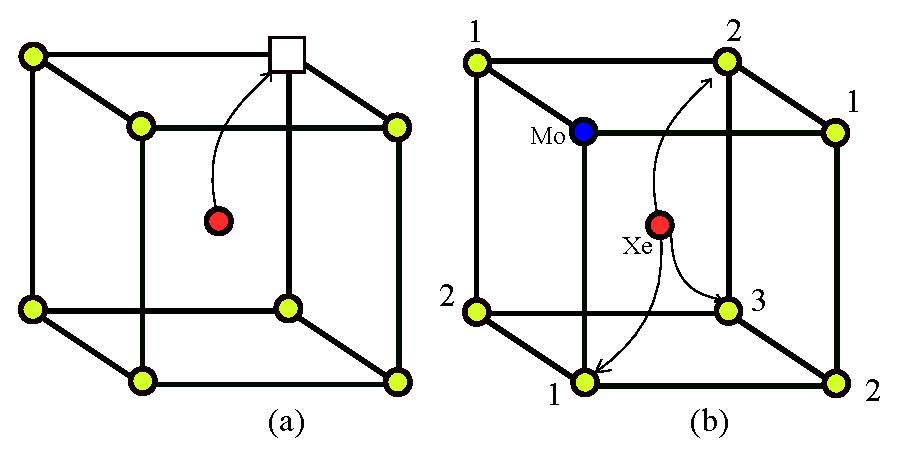
\includegraphics[scale=0.6]{image01}
  \caption{(a)~Diagram of a xenon jump from the centre site to a
    nearest-neighbour vacancy in \textgamma-uranium.
    (a)~All eight jumps are symmetrically equivalent with no molybdenum
    present;
    (b)~with one molybdenum atom in the nearest neighbour shell, there are
        three unique solute jumps (1, 2, and~3).}
    \label{figure01}
\end{figure}

\begin{figure}
    \centering
    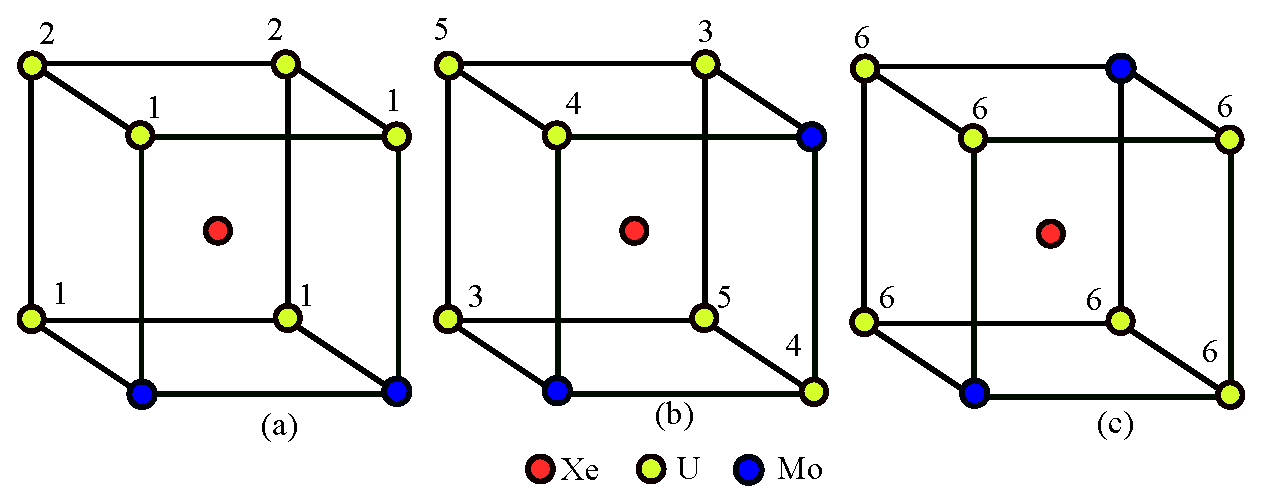
\includegraphics[scale=0.6]{2mo-1xe}
    \caption{The three sets of symmetrically-inequivalent hops of xenon from the centre
        with two molybdenum atoms in the nearest-neighbour shell.
        The numbers denote symmetrically distinct pathways.}
    \label{figure02}
\end{figure}

\begin{figure}
    \centering
    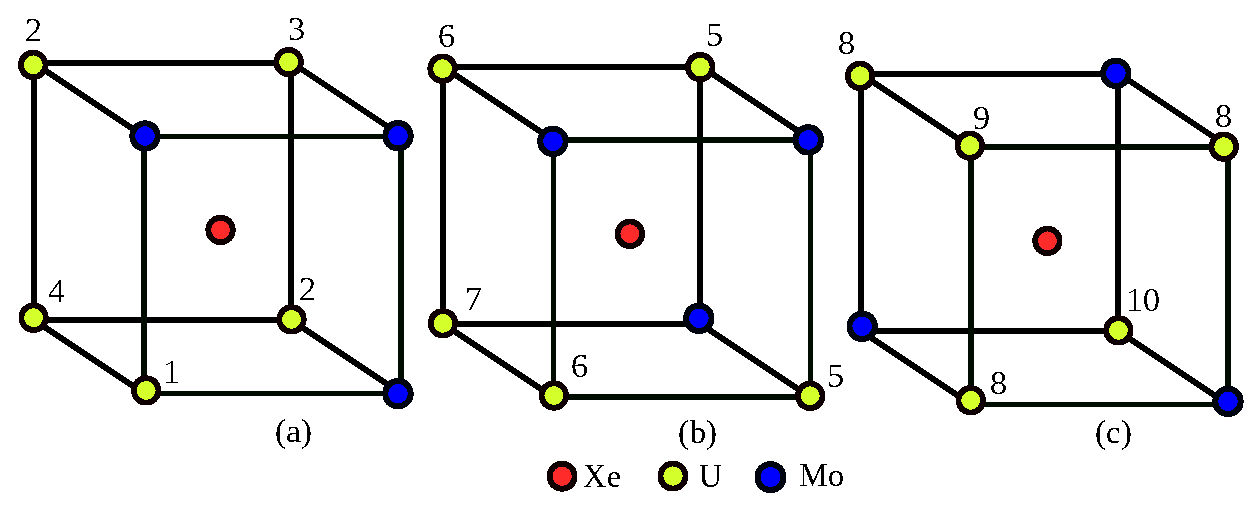
\includegraphics[scale=0.6]{3mo-1xe}
    \caption{The three sets of symmetrically-distinct hops from the centre site
        with three molybdenum atoms in the nearest-neighbour shell. The numbers denote symmetrically distinct pathways.}
    \label{figure03}
\end{figure}

\begin{table}
    \caption{Xenon migration energy ($E_m$) for different configurations.}
    \label{tab_acten}
    \centering
    \begin{minipage}{19.45em}
    \begin{tabular}{ l l l }
      \toprule
        Composition\footnote{The eight nearest-neighbour sites consist of
            one vacancy plus the atoms listed, with the remaining sites
            occupied by uranium atoms.}
        & Xe Jump
        & $E_m$ (eV) \\
      \midrule
        7 U & \hkl<111>~(Fig.~\ref{figure01}a) & 0.161  \\
        1 Mo & 1~(Fig.~\ref{figure01}b) & 0.313 \\ 
             & 2~(Fig.~\ref{figure01}b) & 0.172 \\
             & 3~(Fig.~\ref{figure01}b) & 0.261 \\
        2 Mo & 1~(Fig.~\ref{figure02}a) & 0.110 \\
             & 2~(Fig.~\ref{figure02}a) & 0.212 \\
             & 3~(Fig.~\ref{figure02}b) & 0.532 \\
             & 4~(Fig.~\ref{figure02}b) & 0.108 \\
             & 5~(Fig.~\ref{figure02}b) & 0.224 \\
             & 6~(Fig.~\ref{figure02}c) & 0.110 \\
 	3 Mo & 1~(Fig.~\ref{figure03}a) & 0.515 \\
	     & 2~(Fig.~\ref{figure03}a) & \tiny{\textcolor{purple}{still running}}		\\
	     & 2$^\prime$~(Fig.~\ref{figure03}a) & 0.917	\\
	     & 3~(Fig.~\ref{figure03}a) & 0.579	\\
	     & 4~(Fig.~\ref{figure03}b) & 0.201	\\
	     & 5~(Fig.~\ref{figure03}b) & 0.384	\\
	     & 6~(Fig.~\ref{figure03}b) & 0.386	\\
	     & 7~(Fig.~\ref{figure03}c) & 1.213	\\
	     & 8~(Fig.~\ref{figure03}c) & \tiny{\textcolor{purple}{still running}}	\\
	     & 9~(Fig.~\ref{figure03}c) & \tiny{\textcolor{purple}{still running}}	\\
      \midrule
             & Mo Jump & $E_m$ (eV) \\% \hline
      \midrule
        7 U & \hkl<111>~(Fig.~\ref{figure01}a)  & 2.067 \\
      \bottomrule
    \end{tabular}
    \end{minipage}
\end{table}



\section{Conclusions}
We calculated solute--vacancy binding energies for different solutes in bcc
uranium. Uranium shows relatively high vacancy--solute binding energies compared to iron and aluminium. The unstable nature of \textgamma-U at low temperature contributes to a significant increase in solute--vacancy binding energy relative to other bcc metals. The higher elastic binding energy in bcc uranium produces a high solute--vacancy binding energy.

We also calculated migration energies of xenon and molybdenum in pure bcc
uranium. Molybdenum's migration energy is very high compared to that of xenon,
indicating that in pure bcc uranium, xenon moves much faster than molybdenum.
The relatively low diffusivity of molybdenum also supports our assumptions that molybdenum is randomly distributed in uranium--molybdenum alloys.
We also studied migration energies of xenon in the presence of molybdenum in
\mbox{U--Mo} alloys.
Different combinations of molybdenum in the nearest neighbour and xenon's
distinct jump paths are identified and studied.
A combinatorial analysis suggests that having up to three molybdenum atoms in
the nearest-neighbour shell is highly probable in U-10Mo and U-7Mo alloys.
The presence of molybdenum in the nearest neighbour shell of a xenon atom has
an impact on the migration energy, but it does not generally increase or
decrease the migration energy; both the location of the molybdenum atoms and
direction of the jump influence the migration energy.
Having one molybdenum atom in the nearest-neighbour shell increases the
activation energy between 0.01~eV and 0.15~eV, depending on the location of
the molybdenum atom relative to the xenon atom and the vacancy.
If xenon has two molybdenum atoms nearby, we found a similar increase,
though there are combinations for which the migration energy is lower than it
is in the single-molybdenum cases.
For xenon with three nearby molybdenum atoms,
the migration energy increases for all molybdenum/\allowbreak{}vacancy
arrangements.
While there are several molybdenum arrangements that result in decreased
migration energies relative to some of the two-molybdenum configurations,
the general trend with the addition of molybdenum in the nearest neighbour
shell near xenon is to increase the migration energy, hence reducing xenon
mobility in \mbox{U--Mo} alloys.
 
We did not consider the influence of molybdenum in the second-nearest neighbour
shell in bcc uranium. Future work should include a determination of diffusion
coefficient of xenon using  the kinetic Monte Carlo method.


\bibliographystyle{unsrt}
\bibliography{abbreviated,umox}


